\documentclass[11pt]{article}
\usepackage[letterpaper,margin=1in]{geometry}
\usepackage{color}
\usepackage[dvipdfmx]{graphicx}
\usepackage{amsbsy}
\usepackage{amsmath}
\usepackage{adjustbox}
\usepackage{url}

\newcommand{\argmax}{\mathop{\rm arg~max}\limits}

\begin{document}
\title{Analysis Report on Assignment 6: Feature Engineering}
\author{Yoshinari Fujinuma (Kaggle username: yofu1973)}
\date{}
\maketitle

\section{Preprocessing}
As mentioned in \cite{Boyd-Graber:Glasgow:Zajac-2013}, stemming is a useful preprocessing to normalize input words.

Many sentences in the training data include the sequence ``(SEASON\_NUMBERxEPISODE\_NUMBER)''. 
To let the model understand that this input is equivalent to ``episode NUMBER'' and ``season NUMBER''.
Episode normalization.

Also, we mask the numbers to ``\_\_DIGIT\_\_''.

\section{Feature Engineering on the L2 regularized Logistic Regression}

Strategy:
\begin{enumerate}
 \item Include both generalizable and meaningful feature 
 \item Avoid unmeaning feature to avoid confusing during the training
\end{enumerate}


%Held out dev dataset.
Out of the 14,000 training examples, the first 10,000 examples are used during the training, the rest of 4,000 examples are used as the held out development dataset.

Features:
\begin{enumerate}
 \item unigram
 \item bigram
 \item trope names
 \item word embeddings
 \item named entity 
 \item Genre of the movie (From IMDB\footnote{ftp://ftp.fu-berlin.de/pub/misc/movies/database/genres.list.gz})
\end{enumerate}

After including enough all features except for unigrams and throwing away the unigram feature, the accuracy of the prediction increased.

In the initial trial and errors, and looking into Jorndan's paper, some unigrmas such as ``kill'', ``death'' so even after we drop unigram features, we add them back to the model.

\begin{table}[h]
  \centering
  \begin{tabular}{|l|l|r|r|r|r|}
  \hline \bf Feature        & \bf Held out Accuracy     \\ \hline
   All                      & 0.6797 \\ \hline
   All - unigrams           & 0.6839 \\ \hline
   All - bigrams            & 0.6906 \\ \hline
   All - trope names        & 0.6762 \\ \hline
   %All - word embeddings    & X \\ \hline
   All - Genre of the movie & 0.6615 \\ \hline
   All - Named entity       & 0.6354 \\ \hline
  \end{tabular}
  \caption{\label{feature_importance}Analysis of the importance of features by excluding one by one.}
\end{table}

According to Table \ref{feature_importance}, Named entity features is the most importnat feature. 

I tried including word2vec features by including each dimension of the word vector as a feature. 

Note that when I exclude both bigrams and unigrams, the held out accuracy was $0.6829$ 

\section{Error Analysis}

We analyze the setting when the features are ``All - bigrams'' since it scored highest in the held out dataset.

Second episode.

The word ``kill'' or death-related words gets too high scores. 

Tropes that includes kill or death.


%The following two graph shows the relationship between training examples and accuracy:
%\begin{figure}[htb]
%  \begin{center}
%   \begin{tabular}{c}
%
%    \begin{minipage}{0.5\hsize}
%     \begin{center}
%     \scalebox{0.33}
%      {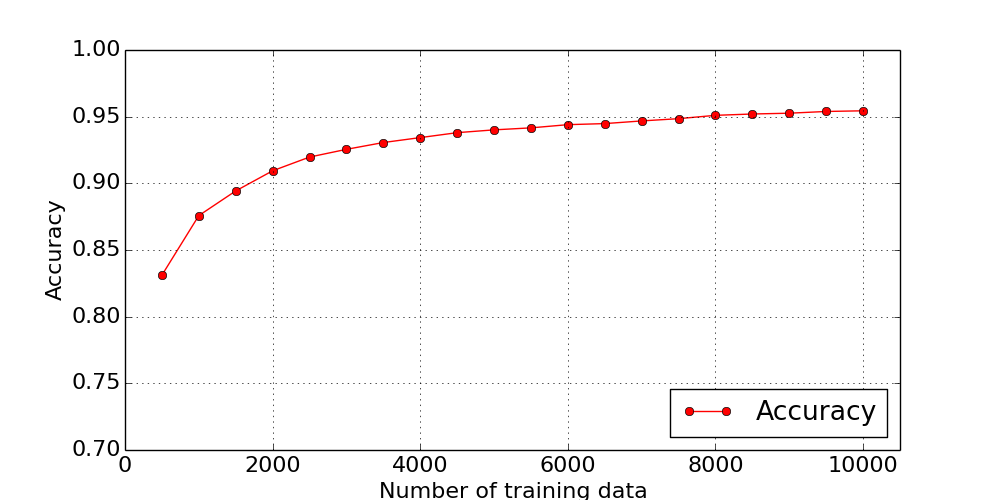
\includegraphics[]{figure_1.png}}
%   
%      \caption{The relationship between the number of training examples and accuracy. The value of $k$ is fixed to $3$. }
%      \label{fig:corpus_size}
%     \end{center}
%    \end{minipage}
%
%    \begin{minipage}{0.01\hsize}
%    \end{minipage}
%
%    \begin{minipage}{0.5\hsize}
%     \begin{center}
%      \scalebox{0.33}
%      {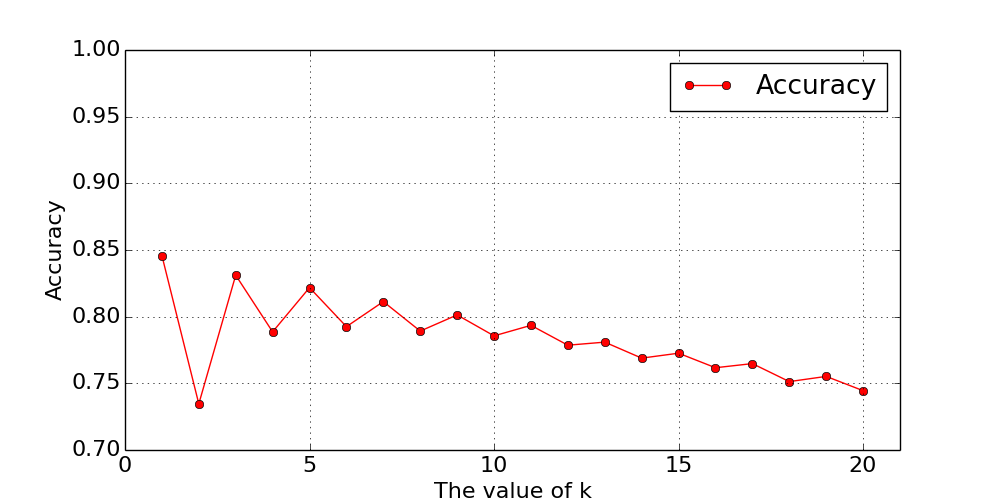
\includegraphics[]{figure_2.png}}
%      \caption{\label{k_and_accuracy}The relationship between $k$ and accuracy. The value of the number of training examples is fixed to $500$}
%     \end{center}
%    \end{minipage}
%
%  \end{tabular}
% \end{center}
%\end{figure}
\bibliographystyle{plain}
\bibliography{analysis}

\end{document}

